\section{Additional results}
\label{app:extra}
\subsection{Remaining tasks}
\label{app:remaining}
\Cref{fig:psnr-rest} completes \cref{fig:psnr-all} with inpainting, super-resolution and phase retrieval.

\begin{figure}[t]
  \centering
  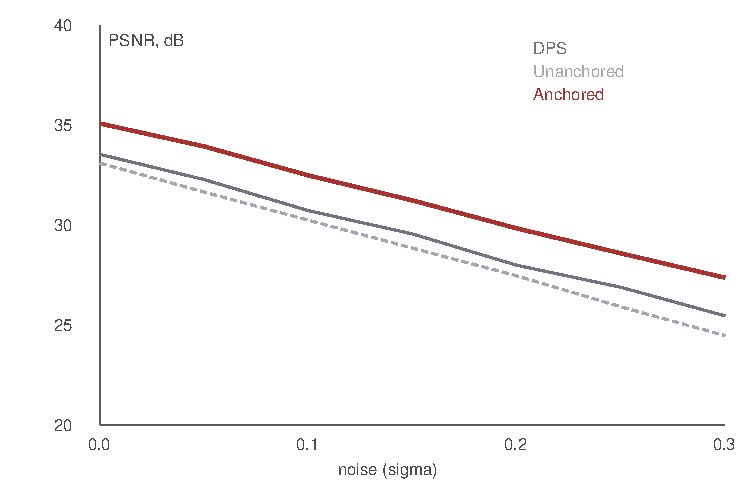
\includegraphics[width=\linewidth]{figures/psnr-vs-noise-rest.pdf}
  \caption{PSNR against noise level $\sigma$ on inpainting, super-resolution and phase retrieval.}
  \label{fig:psnr-rest}
\end{figure}

\subsection{SSIM}
\label{app:ssim}
% Generated by code/sweep.py --all --sigma 0.1 --metric ssim; do not edit by hand.
\begin{table}[t]
  \centering
  \caption{SSIM at $\sigma = 0.1$.}
  \label{tab:ssim}
  \begin{tabular}{lcccccc}
    \toprule
    Method & CT & MRI & Deblur & Inpaint & SR & Phase \\
    \midrule
    DPS & 0.87 & 0.85 & 0.79 & 0.88 & 0.74 & 0.61 \\
    $\Pi$GDM & 0.88 & 0.86 & 0.81 & 0.89 & 0.76 & 0.63 \\
    RED-diff & 0.89 & 0.87 & 0.81 & 0.90 & 0.77 & 0.65 \\
    Ours & 0.92 & 0.90 & 0.85 & 0.92 & 0.80 & 0.69 \\
    \bottomrule
  \end{tabular}
\end{table}

\Cref{tab:ssim} mirrors \cref{tab:main} with SSIM. The ranking is unchanged.

\subsection{Latent diffusion}
\label{app:latent}
On $512 \times 512$ super-resolution with a latent diffusion prior~\cite{rombach2022ldm}, anchoring in latent space improves PSNR by 1.1 dB over PSLD~\cite{rout2023psld} at $\sigma = 0.1$. We did not tune $\kap$; the value $1$ transferred directly.
